\chapter{Evaluation and Analysis}\label{sec:results}

The scripts that perform the evaluation of our testing set, are
\texttt{evaluation.sh} and \texttt{exec\_query.sh}.

The values of parameters of the \texttt{KDTree} described in \Cref{sec:KD} used are:

\begin{itemize}
    \item $\omega = \{2,3,5,10,20\}$
    \item $\kappa$ gets computed based on $\omega$ factors (s.t. $\kappa - 1$
        has to be a factor of $\omega$).
    \item $\mu$ = 1 (Average Bitrate Mode)
    \item $\delta = \pm 25 bps$
    \item $\rho$ = 0.99
\end{itemize}

\section{Video Identification} 

After receiving a list of matching windows from the KD-Tree, we classify each
one of them as a proper \textbf{match} iff the window's ID matches the ID of
the capture we passed to the Java identification process, whereas, if the ID of
the capture and the window ID are different, we classify the returned window as
a \textbf{mismatch}.

We then report, for various $\omega$ window sizes, the accuracy of our method,
to be the proportion of matches with respect to the number of mismatches over
the total number of returned windows as:

Let $n$ be the number of returned windows for a given capture trace, and let
$TP$ represent the number of matches, and $FP$ to represent the number of
returned mismatches:

It follows that $n = TP + FP$

\begin{equation*}
    \mathbf{acc} = \dfrac{TP}{n} = 1 - \dfrac{FP}{n}
\end{equation*}

As mentioned in \Cref{sec:testing}, our testing dataset consists of the same
100 movies present in the database at 8 unseen enforced bandwidths. We pass
each capture to the identification process, that runs the evaluation by varying
the window size $\omega$, and the corresponding key size $\kappa$. For every
run, we then compute the number of matches/mismatches, and report the
statistics shown in \Cref{lst:stats}. In addition, we plot for each
configuration the number of matches, the number of collisions and the number of
mismatches. The number of collisions, represents the number of matches from
different bandwidth levels, (e.g. suppose to have a capture at 6.0 \emph{Mbps},
now assume the KDTree returns as matching windows, a list of matches all of the
same movie, but at different bandwidths, 5.0 \emph{Mbps}, and 7 \emph{Mbps},
then the number of collisions is 2).

\begin{figure}[!h]
  \centering
  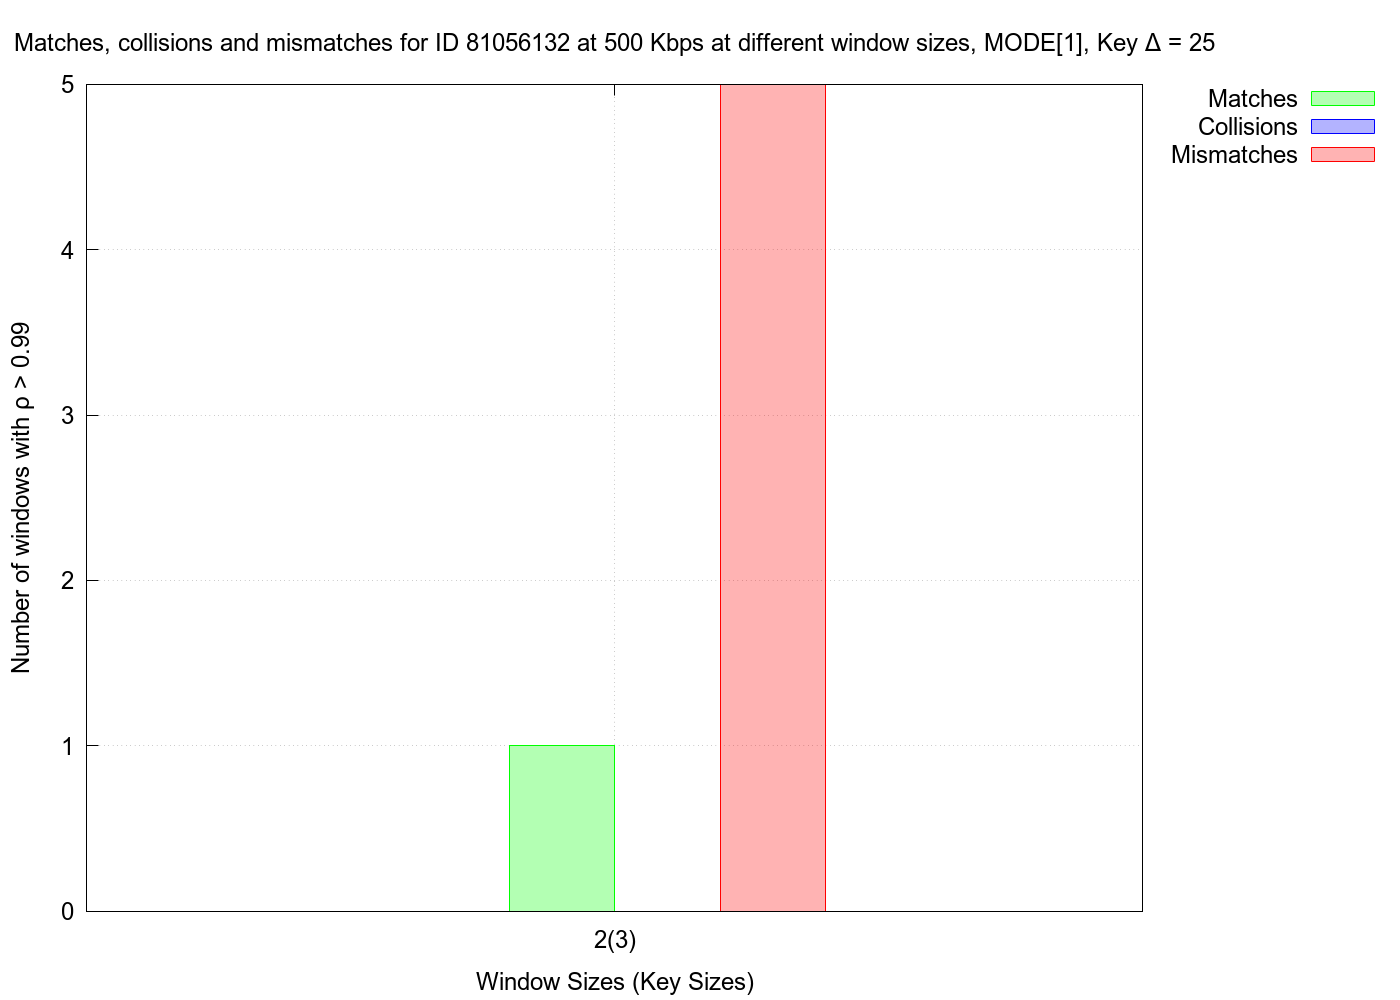
\includegraphics[width=\columnwidth]{img/acc_81056132_500.png}
  \caption{Frequency of matches, collisions, and mismatches  at various window
  sizes for "Dirty John" ID: 81056132, recorded at 500 Kbps}
  \label{fig:matches_1}
\end{figure}
\begin{figure}[!h]
  \centering
  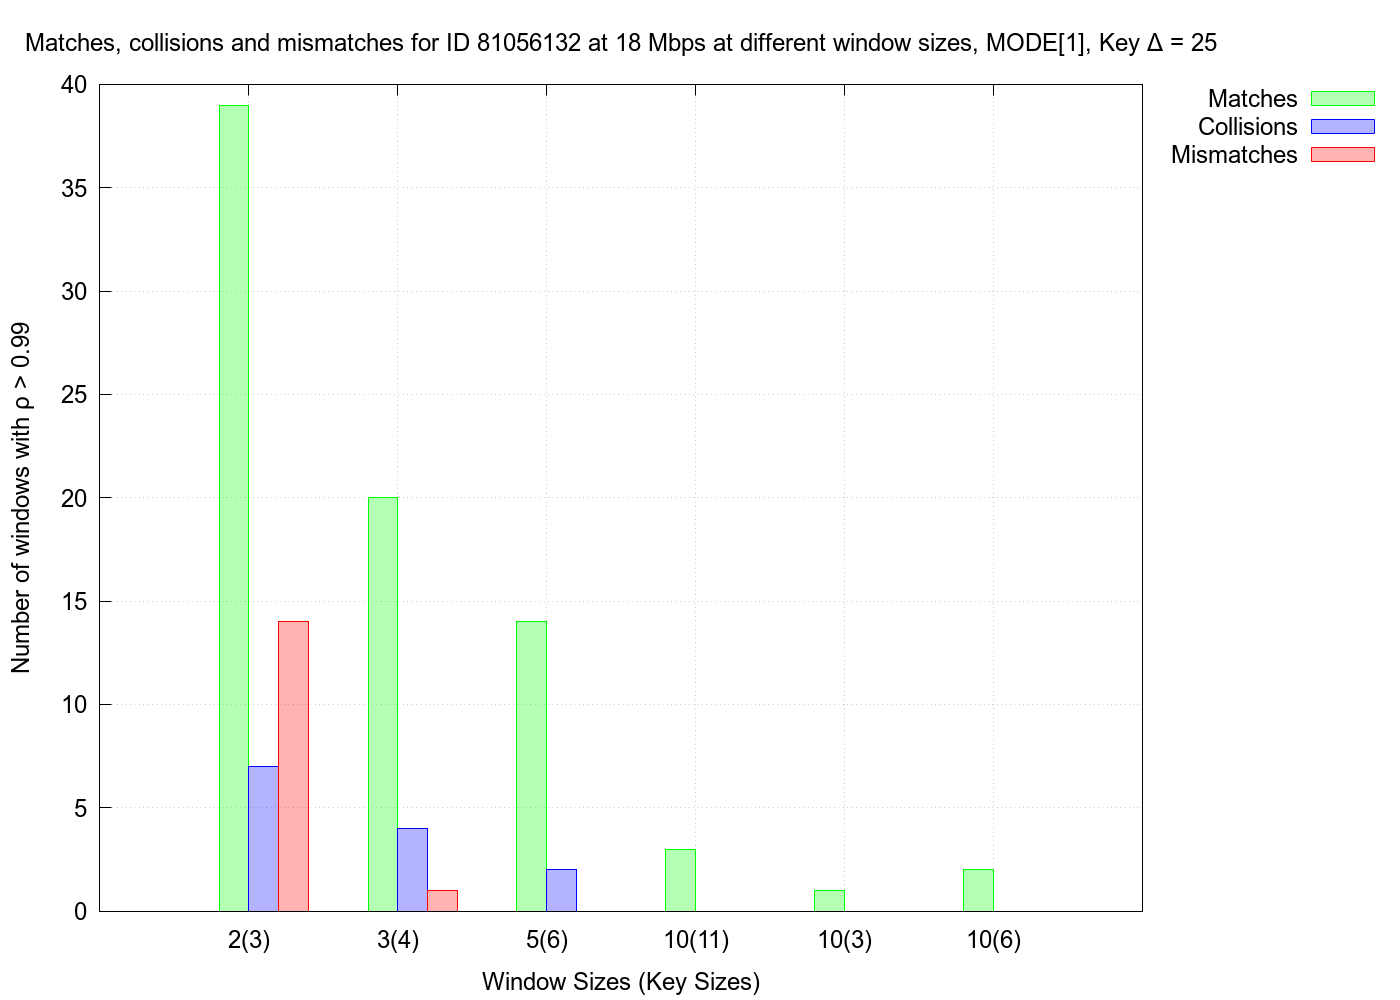
\includegraphics[width=\columnwidth]{img/acc_81056132_18000.png}
  \caption{Frequency of matches, collisions, and mismatches  at various window
  sizes for "Dirty John" ID: 81056132, recorded at 18 Mbps}
  \label{fig:matches_2}
\end{figure}

The plot in \Cref{fig:matches_1} represent a low-bandwidth capture where the
number of mismatches dominates the number of matches. The fact that with a
small window the KD-Tree returns a greater numnber of mismatches then when
considering larger windows is trivial, since the search key is based on the
average bitrate. Despite this, the KD-Tree, does not return matches nor
mismatches for $\omega = \{3, 5, 10, 20\}$.  We observe this behavior only in
low-bandwidths scenarios, and it is due to an incorrect segment size inference
by adudump. The main reason for why adudump cannot correctly inference the
video segment sizes is spottable by  by looking at the trace in
\Cref{lst:adutrace}, particularly at the destination IP address (which is the
local address of the interface we are recording traffic on). One can notice how
ADUs have different \texttt{PORT} numbers, one for every virtual connection
established by the the custom TCP-connection algorithm running on OCAs. On
contrary, in \cite{netflix-real-time}, the reported adudump traces did not
manifest this behavior.

In \Cref{fig:matches_2}, at a much higher bandwidth shows how the number of
matches varies as increasing $\omega$. We note how for $\omega=20$ the KD-Tree
does not return any match nor mismatch. In \Cref{tab:matches} we report the
overall number of matches/mismatches for different $\omega$s.

\begin{longtable}{|c c c|}
\caption{Frequency of matches for different values of $\omega$}\label{tab:matches}\\
\hline
$\omega(\kappa)$ &
\textbf{Matches} &
\textbf{Mismatches} \\
\hline
\endhead
\hline
\endfoot
2(3)	& 17648	& 6794 \\
3(4)	& 12957	& 410 \\
5(6)	& 6414	& 2 \\
10(11)	& 1541	& 0 \\
10(2)	& 1481	& 0 \\
10(3)	& 1516	& 0 \\
10(6)	& 1528	& 0 \\
15(16)	& 461	& 0 \\
15(2)	& 461	& 0 \\
15(4)	& 459	& 0 \\
15(6)	& 456	& 0 \\
20(11)	& 138	& 0 \\
20(21)	& 138	& 0 \\
20(2)	& 145	& 0 \\
20(3)	& 137	& 0 \\
20(5)	& 139	& 0 \\
20(6)	& 142	& 0 \\
\hline
\textbf{TOTAL} & 45761 & 7206 \\
\multicolumn{2}{|l}{\textbf{ACCURACY}} & 0.86 \\
\end{longtable}

\section{Bitrate Ladders}

At first, we evaluate the accuracy of the reconstruced bitrate ladders by
computing the RMSE between each one and its corresponding HAR-based bitrate
ladder. We have decided to use the RMSE, as it is a well-known indicator that
aggregates the residuals to give a measure of the magnitude of error in our
predictions, and it is computed as follows.

Let $Y=\{y_1, y_2 \dots y_n\}$ be the set of HAR-based bitrates for movie $m$,
at enforced bandwidth $b$, and let $\hat{Y}=\{\hat{y}_1, \hat{y}_2 \dots
\hat{y}_n\}$ be the set of ADU-based computed bitrates for the same movie at
the same enforced bandwidth, then:

\begin{equation*}
    \mathbf{RMSE_{m, b}} = \sqrt{\dfrac{\Sigma_{i=0}^{n}(y_i - \hat{y}_i)^2}{n}}
\end{equation*}

where $n = |Y| = |\hat{Y}|$

Then, the \emph{mean-normalized} RMSE is given by:

\begin{equation*}
    \mathbf{NRMSE_{m, b}} = \dfrac{RMSE_{m, b}}{\overline{\hat{y}}}
\end{equation*}

In addition, in order to assess the uniqueness of both the real and the
reconstrcuted bitrate ladders, we compute, for each bitrate ladder, its average
bitrate, the bitrate standard deviation, and the median. 

\begin{figure}[!h]
  \centering
  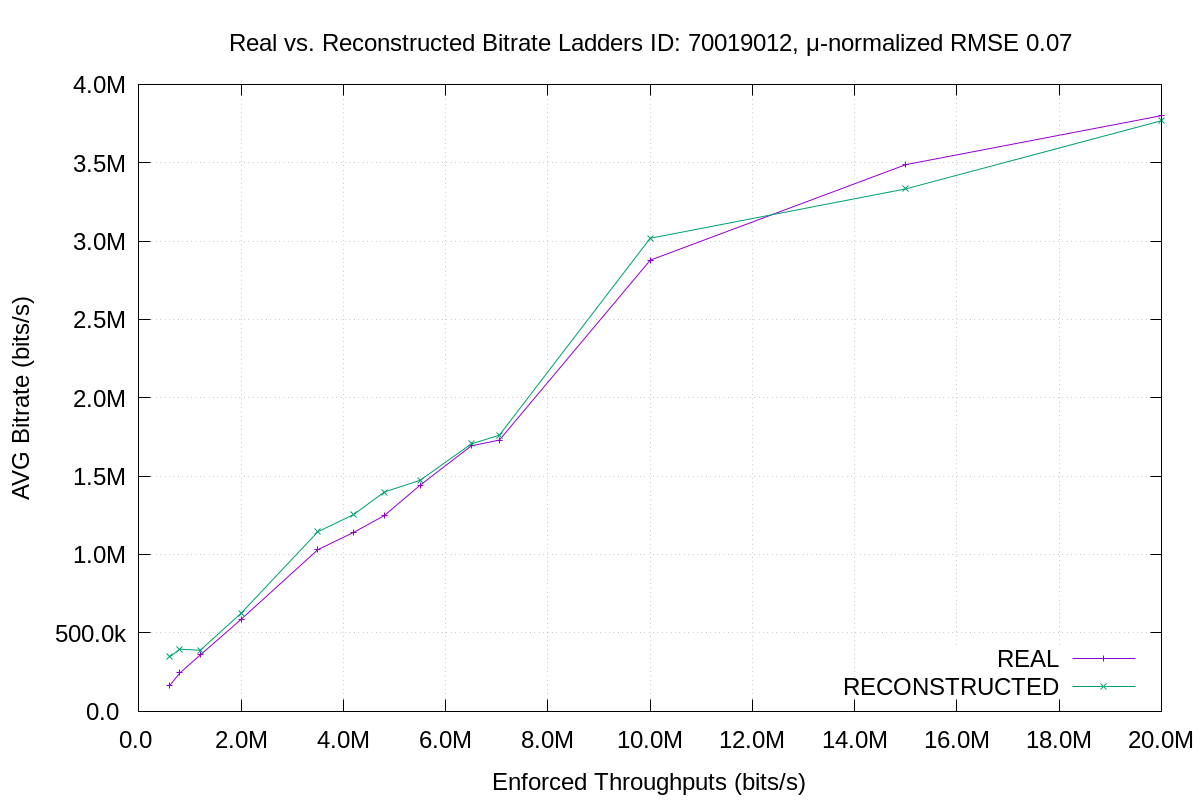
\includegraphics[width=\columnwidth]{img/70019012.png}
  \caption{Comparison between the HAR-based bitrate ladder (REAL) and the
  ADU-based reconstructed bitrate ladder for "Casino" ID: 70019012. Accuracy of
  reconstruction is shown as the RMSE.}
  \label{fig:bl_comparison_good}
\end{figure}

The plot above represents the "real" and reconstructed bitrate ladders.  The
accuracy of our prediction is represented by the RMSE, which is 0.07.  This
title's bitrate ladder gets reconstructed faithfully, and almost every title in
our database follow this trend. This is confirmed by further looking at the
average RMSE shown at the end of \Cref{tab:bitrate_ladders_stats}. Eventually,
63 titles have an RMSE less than 0.12, and 87 less than 0.16.
\Cref{fig:bl_comparison_good_1} and \Cref{fig:bl_comparison_good_2} are two
examples of reconstruction which RMSE is 0.12 and 0.16 respectively.

\begin{figure}[H]
  \centering
  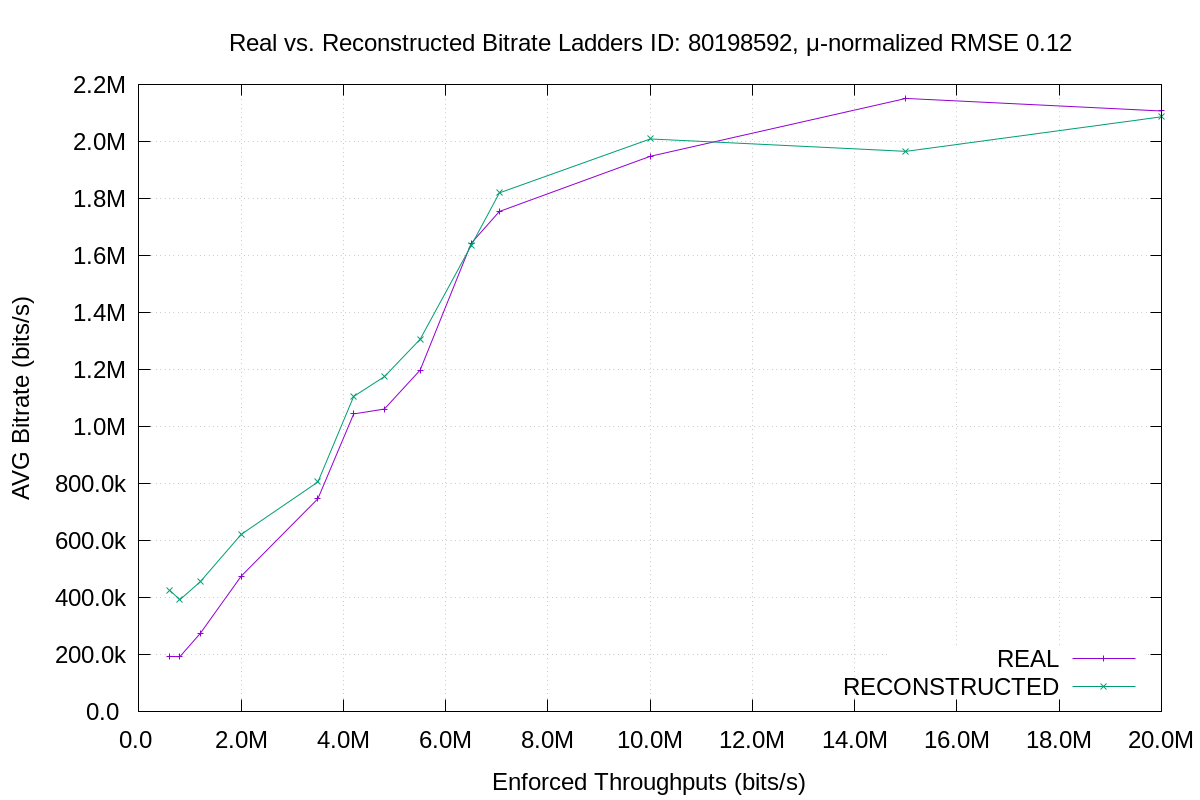
\includegraphics[width=\columnwidth]{img/80198592}
  \caption{Comparison between the HAR-based bitrate ladder (REAL) and the
  ADU-based reconstructed bitrate ladder for "Armed Response" ID: 80198592.
  Accuracy of reconstruction is shown as the RMSE.}
  \label{fig:bl_comparison_good_1}
\end{figure}

By looking at the above plot we spot two major areas where the differences
between the real and the reconstructed bitrates have greater impact on the
overall accuracy. Bottom left, when the enforced bandwidth and the bitrates are
low, and top right, at 15\emph{Mbps}. We focus our attention on the bottom-left
area, and notice how it correlates with the RMSE of the following plots.

\newpage
\begin{figure}[H]
  \centering
  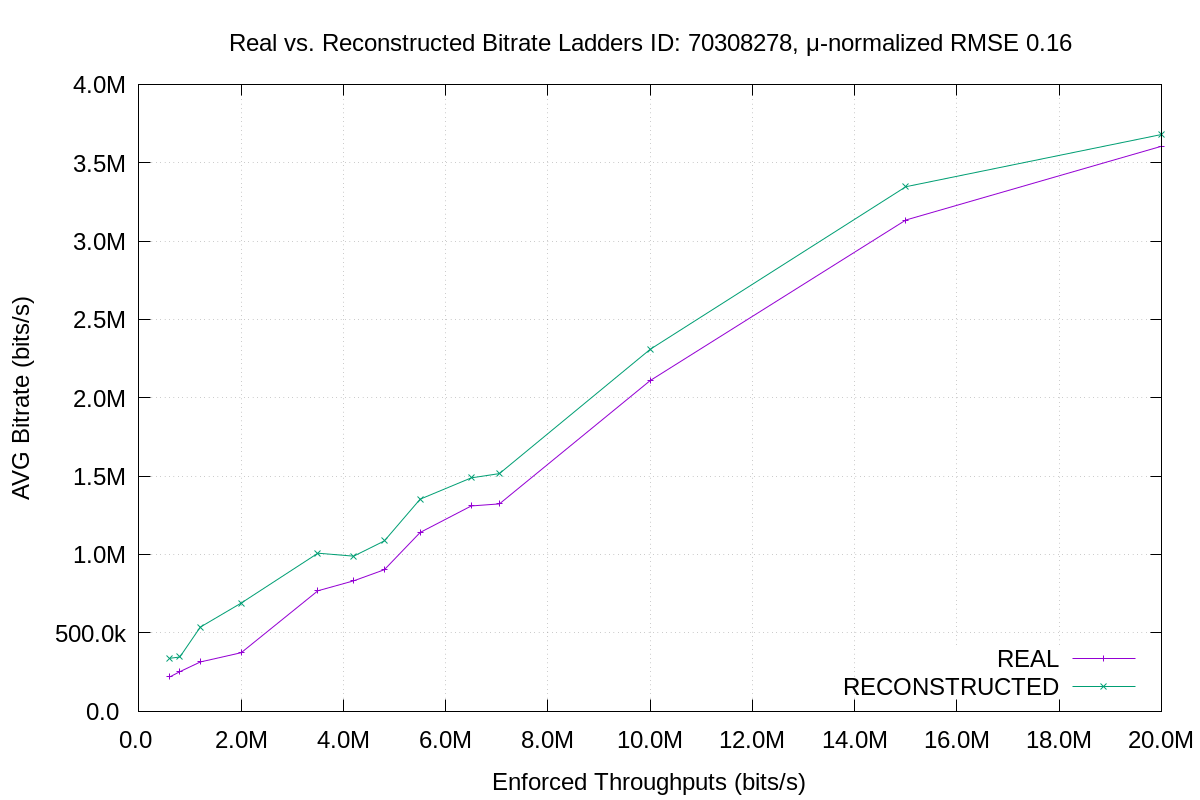
\includegraphics[width=\columnwidth]{img/70308278}
  \caption{Comparison between the HAR-based bitrate ladder (REAL) and the
  ADU-based reconstructed bitrate ladder for "Mission Blue" ID: 80198592.}
  \label{fig:bl_comparison_good_2}
\end{figure}

In this case we observe that with a greater RMSE, the two curves start to be
parallel to each other. By looking at the plot in \Cref{fig:bl_comparison_bad}
we see a magnified version of this behavior, and explain its existence.

\begin{figure}[!h]
  \centering
  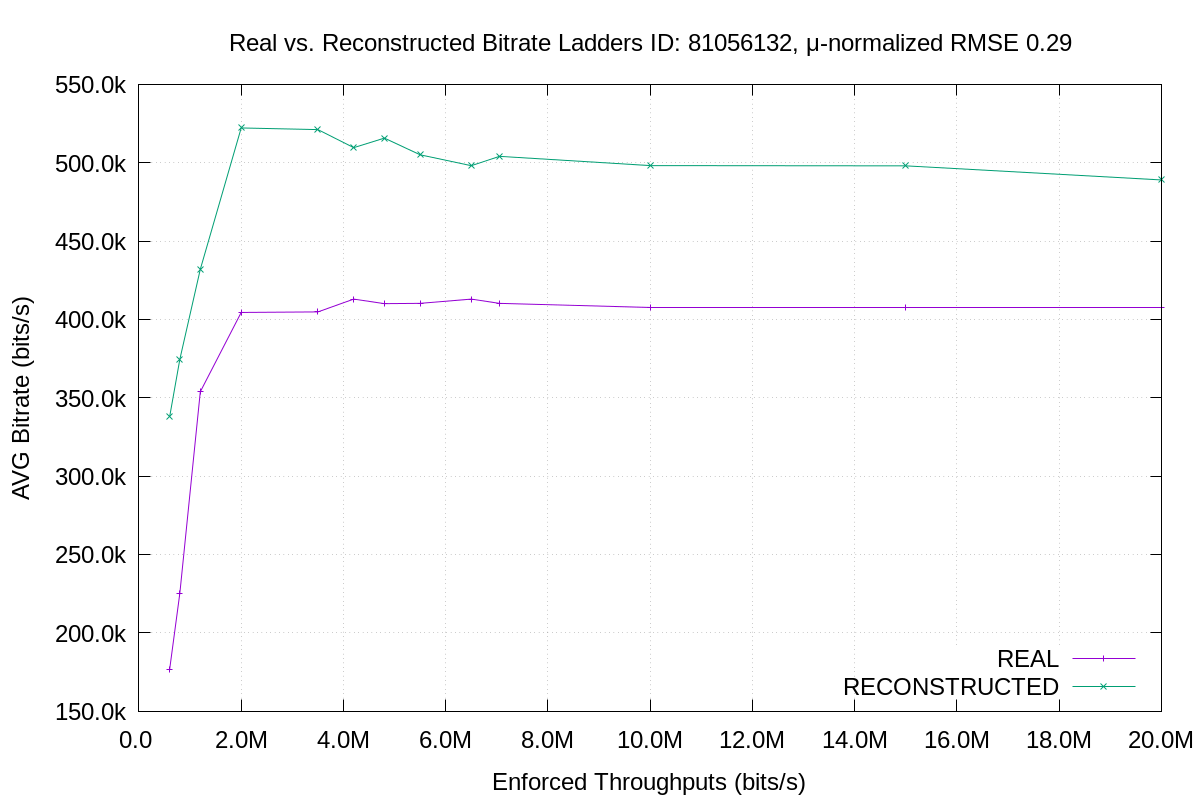
\includegraphics[width=\columnwidth]{img/81056132.png}
  \caption{Comparison between the HAR-based bitrate ladder (REAL) and the
  ADU-based reconstructed bitrate ladder for "Dirty John" ID: 81056132.}
  \label{fig:bl_comparison_bad}
\end{figure}

This plot represents a particular case of a recontruction which RMSE we
consider too high. This behavior, as already mentioned in the description of
\Cref{fig:matches_1}, happens only at low-enforced bandwidth, in this
particular case one can observe how the "real" bitrate ladder, has also a low
average bitrate in comparison with the one seen so far. That in turns confirm
that our identification method is prone to error when a Netflix title has been
encoded at low bitrates, or in poor network conditions.

\subsection{Uniqueness of Bitrate Ladders}

We have collected the statistics in \Cref{tab:bitrate_ladders_stats}, to show
that for our set of titles, each ladder is indeed unique. In fact, each ladder,
can be modeled as a Gaussian Probability Distribution with mean $\mu$ and
standard deviation $\sigma$. Across our entire database these two values are
unique, therefore we can conclude that each bitrate ladder is unique.o

In addition to that, we have implemented a simple K-means clustering script,
which we feed the \emph{reconstructed} $\mu$, $\sigma$ of all video titles
captured at 20Mbps and median $\tilde{y}$.  Following we present the plot
obtained by setting the number of centroids $K = 10$, (as the number of
different movie genres in our database), that shows a possible labeling based on
the average bitrate $\mu$.

\begin{figure}[!h]
  \centering
  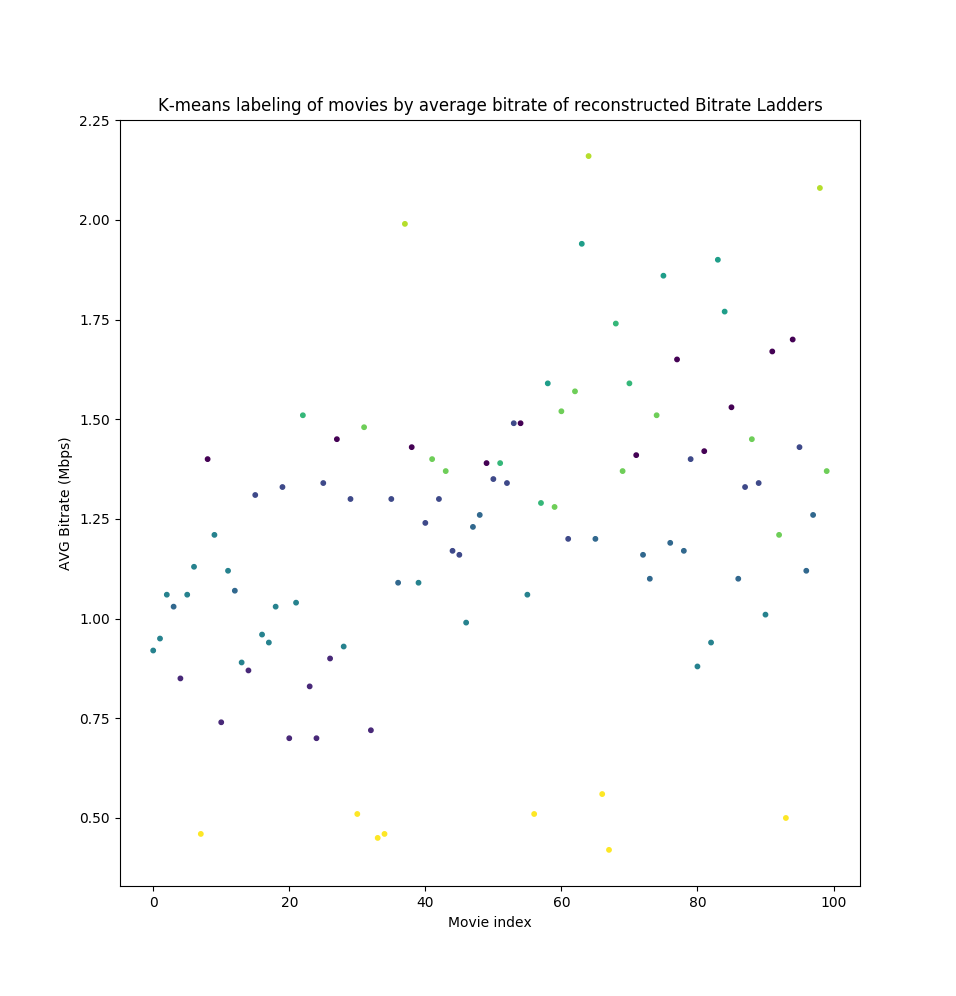
\includegraphics[width=\columnwidth]{img/clusters.png}
  \caption{K-means labeling of average bitrates for every reconstructed bitrate
  ladder.}
  \label{fig:clusters}
\end{figure}

Below we show a magnified and labeled version of the result given by the
clustering. Interestingly, we notice how despite movies with approximately
close average bitrates can be assigned to different clusters, as standard
deviation, median, and RMSE may be crucial in the discrimination of the cluster
appropriate custer. 

The red stroke polygon encloses an area of particular
interest, for which the average bitrate of 6 out of 10 cartoons in our database
varies by less than 200 \emph{Kbps}. 

We notice also how  4 out of 10 cartoons in our database get clustered together
with this setting (\emph{Madagascar 3}, \emph{Despicable Me 2}, \emph{Minions},
and \emph{The Emoji Movie}), as the complexity of the scenes across them may
potentially be alike. 

\begin{figure}[!h]
  \centering
  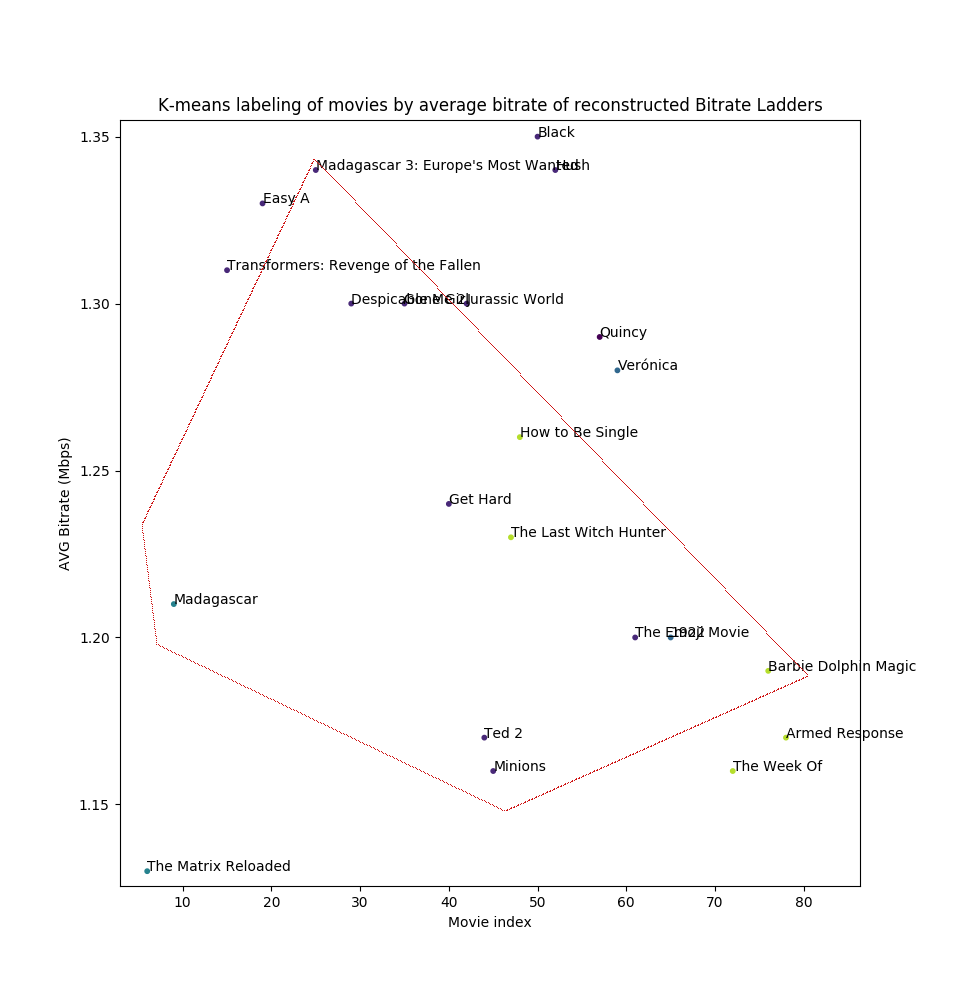
\includegraphics[width=\columnwidth]{img/zoomed.png}
  \caption{Zoomed version of \Cref{fig:clusters}, displaying the title of each movie}
  \label{fig:zoomed}
\end{figure}
